\documentclass[11pt]{scrbook}
%\usepackage[top=10mm,bottom=60mm,left=25mm,right=25mm, a4paper]{geometry}
%\usepackage[pass]{geometry}
%\newgeometry{left=5cm,right=5cm,top=0in,bottom=1.5cm, %left is inner
%    marginparsep=5mm,marginparwidth=30mm,
%    headheight=20mm,headsep=1cm,
%    footskip=1.5cm}

\usepackage{microtype,soul,filecontents,pifont,booktabs,url}
\usepackage[usenames,dvipsnames,svgnames]{xcolor}
\usepackage{amsmath,etoolbox}
 \usepackage{pgf,fp}
\usepackage{tikz}
\usepackage{picture}
\usepackage{lettrine,caption,multicol}

\usepackage{lipsum,soul}
%\usepackage{palatino}
\usepackage{calligra}
\usepackage{fourier-orns}
%\usepackage[T1]{fontenc}
\usepackage{eso-pic}
\usepackage{layouts}
\usepackage{alphalph}
\usepackage{caption}
\usepackage{fmtcount}
\usepackage[listings,theorems]{tcolorbox}
%\usepackage[charter]{mathdesign}
% \def\rmdefault{bch} % not scaled
% \def\ttdefault{blg}
\usepackage{filecontents,ragged2e,changepage}
\makeatletter
%% decide on fonts
\IfFileExists{ifxetex.sty}{%
  \RequirePackage{ifxetex}}{}
  \ifxetex
     \usepackage{fontspec}
     \defaultfontfeatures{Mapping=tex-text}
     \setmainfont{Linux Libertine G}
     %\setsansfont{Georgia}
  \else
     \usepackage{mathpazo}
     \usepackage[T1]{fontenc}
  \fi


% Define some shortcut macros for error/warning/info logging.

\newcommand{\athenawarning}[1]{\PackageWarning{athena}{#1}}
\athenawarning{We are starting on an adventure!}
%

%\usetikzlibrary{decorations.markings}
%\usepackage{doc}
%\usetikzlibrary{calc} 
\usetikzlibrary{decorations,decorations.shapes,shapes,fadings,patterns}
     % We need lots of libraries...
        \usetikzlibrary{
          arrows,
          calc,
          fit,
          patterns,
          plotmarks,
          shapes.geometric,
          shapes.misc,
          shapes.symbols,
          shapes.arrows,
          shapes.callouts,
          shapes.multipart,
          shapes.gates.logic.US,
          shapes.gates.logic.IEC,
          circuits.logic.US,
          circuits.logic.IEC,
          circuits.logic.CDH,
          circuits.ee.IEC,
          datavisualization,
          datavisualization.formats.functions,
          er,
          automata,
          backgrounds,
          chains,
          topaths,
          trees,
          petri,
          mindmap,
          matrix,
          calendar,
          folding,
          fadings,
          shadings,
          spy,
          through,
          turtle,
          positioning,
          scopes,
          decorations.fractals,
          decorations.shapes,
          decorations.text,
          decorations.pathmorphing,
          decorations.pathreplacing,
          decorations.footprints,
          decorations.markings,
          shadows,
          lindenmayersystems,
          intersections,
          fixedpointarithmetic,
          fpu,
          svg.path,
          external,
        }



\definecolor{theblue} {rgb}{0.02,0.04,0.48}
\definecolor{thered}  {rgb}{0.65,0.04,0.07}
\definecolor{thegreen}{rgb}{0.06,0.44,0.08}
\definecolor{thelightgreen}{rgb}{0.06,0.44,0.06}
\definecolor{thegrey} {gray}{0.5}
\definecolor{thegray} {gray}{0.5}
\definecolor{thedarkgray} {gray}{0.95}
\definecolor{theshade}{gray}{0.94}
\definecolor{theframe}{gray}{0.75}
\definecolor{thecream}{rgb}{1,0.95,0.4}
\definecolor{spot}{rgb}{0,0.2,0.6}
\definecolor{boxframe}{gray}{0.8}
\definecolor{boxfill}{rgb}{0.95,0.95,0.99}
\definecolor{theoption}{rgb}{0.118,0.546,0.222}
\definecolor{themacro}{rgb}{0.784,0.06,0.176}
\definecolor{ExampleFrame}{rgb}{0.628,0.705,0.942}
\definecolor{ExampleBack}{rgb}{0.963,0.971,0.994}
\definecolor{Hyperlink}{rgb}{0.281,0.275,0.485}
\colorlet{thehyperlink}{theblue}
\newcommand*{\defaultcolor}{\color{black}}
\newcommand*{\spotcolor}{\color{spot}}

\newcommand\lorem{Fusce adipiscing justo nec ante. Nullam in enim.
 Pellentesque felis orci, sagittis ac, malesuada et, facilisis in,
 ligula. Nunc non magna sit amet mi aliquam dictum. In mi. Curabitur
 sollicitudin justo sed quam et quadd. \par}

\pgfkeys{/xpage/.is family}

\def\cxset{\pgfqkeys{/xpage}} %Notice this is pgf q keys
\usepackage{xgeometry}

\begin{document}

\setlength\paperwidth@cx{\paperwidth}
\setlength\paperheight@cx{\paperheight}
\setlength\bindingcorrection{0.25in}



% draw a trial layout based on some values we have passed
\drawtriallayout

\showequations

\printgeometryvalues
\readability

\newpage

\drawtriallayout

\readability

\newpage





\begin{figure}
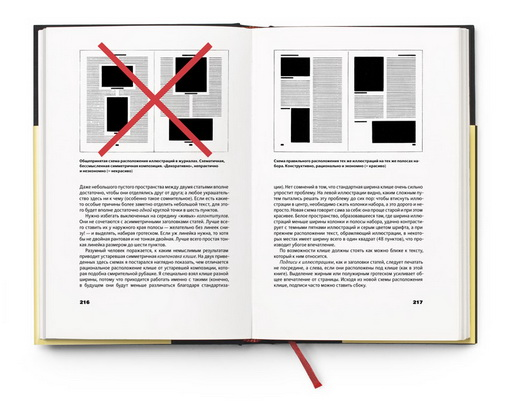
\includegraphics[width=0.95\textwidth]{tchichold01}
\caption{\protect\url{http://www.artlebedev.com/everything/izdal/novaya-tipografika/}}
\end{figure}

%http://www.google.com/imgres?start=245&hl=en&safe=off&sa=X&biw=1310&bih=654&tbm=isch&prmd=imvnso&tbnid=A5938qBinqJLrM:&imgrefurl=http://lovelyligatures.tumblr.com/&docid=DvV3WNMH-kJR6M&imgurl=http://25.media.tumblr.com/tumblr_m3hybzMd7x1ro5iomo1_500.jpg&w=450&h=642&ei=H6mzT4ChO4rYrQf80c32Aw&zoom=1&iact=hc&vpx=384&vpy=256&dur=3610&hovh=268&hovw=188&tx=113&ty=178&sig=101250704487237849374&page=10&tbnh=151&tbnw=106&ndsp=29&ved=1t:429,r:16,s:245,i:155
%
%
%
%


\tikzstyle{activity}=[draw,
                      rectangle,
                      rounded corners, 
                      fill=black!5,
                      thick,
                      minimum width=6cm,
                      minimum height=2.2cm, 
                      text width=5.5cm,
                      >=latex
                      ]
\begin{figure*}
\centering
\begin{tikzpicture}[mystylei/.style={draw,ellipse,rounded corners, fill=gray!23,thick,minimum
width=6cm,minimum height=1cm, text width=5.5cm, ragged , inner sep=3pt}]


%start to define nodes relative to each other
\newcommand\addblock[2]{\node[activity, node distance=0] (#1) {\textsc{\textbf{#1}}. \textsf{#2}};\def\temp{#1}}

\def\addblockbelow#1#2{\node[activity] (#1) [below=of \temp] {#1. \textsf{#2}};\draw[->] (\temp)[>=latex] -- (#1);
\def\temp{#1}
}

\addblock{A1}{Choose paper and font size}
\addblockbelow{A}{Font based. Load .clo file, determine the following parameters based on font.\\
headsep, footskip, topskip, maxdepth.
}
\addblockbelow{B}{Text width.\\ set length to 0.7\textbackslash paperwidth}
\addblockbelow{C}{Adjust for topskip and round to fixed number of lines.}
\addblockbelow{D}{Set outer margin at 0.2 paper width.}
\addblockbelow{D1}{Set inner margin at 0.1 paper width.}
\end{tikzpicture}
\begin{tikzpicture}[mystylei/.style={draw,ellipse,rounded corners, fill=gray!23,thick,minimum
width=6cm,minimum height=1cm, text width=5.5cm, ragged , inner sep=3pt}]


%start to define nodes relative to each other
\newcommand\addblock[2]{\node[activity, node distance=0] (#1) {\textsc{\textbf{#1}}. \textsf{#2}};\def\temp{#1}}

\def\addblockbelow#1#2{\node[activity] (#1) [below=of \temp] {#1. \textsf{#2}};\draw[->] (\temp)[>=latex] -- (#1);
\def\temp{#1}
}

\addblock{A1}{See notes, regarding choice of paper and font based on readability and length of book.}
\addblockbelow{A}{Font based. Load .clo file, determine the following parameters based on font.\\
headsep, footskip, topskip, maxdepth.
}
\addblockbelow{B}{Text width.\\ set length to 0.7\textbackslash paperwidth}
\addblockbelow{C}{Adjust for topskip and round to fixed number of lines.}
\addblockbelow{D}{Set outer margin at 0.2 paper width.}
\addblockbelow{D1}{Set inner margin at 0.1 paper width.}
\end{tikzpicture}
\caption{Workflow for Engineers Instructions and RFI works. All Departments get involved when there is a Change Order. Evaluate Change Orders as they occur and keep contemporaneous records. }
\end{figure*}

%% USER GEOMETRY FIXED TOTALLY
\begin{figure*}
\centering
\begin{tikzpicture}[mystylei/.style={draw,ellipse,rounded corners, fill=gray!23,thick,minimum
width=6cm,minimum height=1cm, text width=5.5cm, ragged , inner sep=3pt}]


%start to define nodes relative to each other
\newcommand\addblock[2]{\node[activity, node distance=0] (#1) {\textsc{\textbf{#1}}. \textsf{#2}};\def\temp{#1}}

\def\addblockbelow#1#2{\node[activity] (#1) [below=of \temp] {#1. \textsf{#2}};\draw[->] (\temp)[>=latex] -- (#1);
\def\temp{#1}
}
\addblock{A1}{Specify paper and font size}
\addblockbelow{A}{System loads .clo files and sets paper parameters.}
\addblockbelow{B}{Specify inner, outer,top, bottom, right, textwidth}
\addblockbelow{C}{calculate reasonable, settings for items that have not been specified.}
\addblockbelow{D}{Issue warnings.}
\addblockbelow{D1}{Write to log all warnings and final dimensions.}
\end{tikzpicture}
\caption{Workflow for Engineers Instructions and RFI works. All Departments get involved when there is a Change Order. Evaluate Change Orders as they occur and keep contemporaneous records. }
\end{figure*}

\begin{table}
\centering
\caption{Octavo page layout parameters, influenced by font-size}
\begin{tabular}{llll}
\toprule
                    & 10pt & 11pt &12pt \\
\midrule
\textit{Octavo}              &      &      &\\
headsep        &  6pt  &  7pt &  8pt\\
topskip          & 10pt &  11pt & 12pt\\
texwidth         &0.7paperwidth & &\\
\midrule
\textit{LaTeX}              &      &      &\\
headsep        & .25in   &  .275in & .275in \\
topskip          & 10pt &  11pt & 12pt\\
footskip         &.35in &  .38in & 30pt \\
maxdepth         &.5\textbackslash topskip & &\\
textwidth        & 345pt  & 360pt & 390pt\\
\bottomrule
\end{tabular}
\end{table}

\end{document}
